\begin{figure}[h]
	\centering
	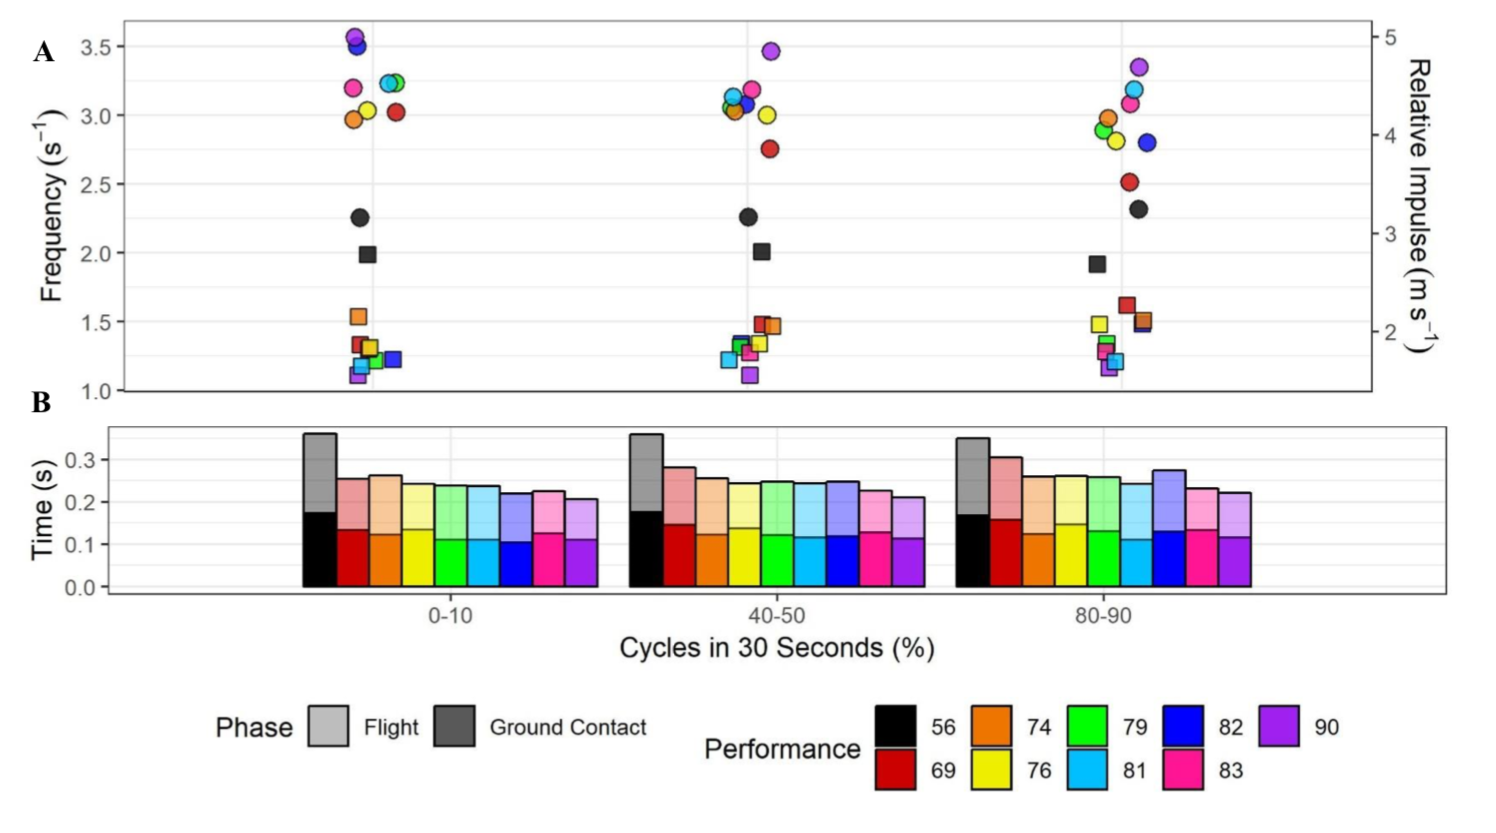
\includegraphics[width=\linewidth]{pix/fig3}
	\label{fig3}
	\caption{Kinetic parameters (ground contact and flight time (B) as well as relative vertical ground reaction force (GRF) impulse of the right foot and skipping frequency (A)) over three phases of the 30 s skipping test, depicted as 10\% intervals of the total number of ground contacts. Circles represent the skipping frequency and squares the relative vertical GRF impulse. Athletes' skipping performance is illustrated in distinct colors.}
\end{figure}